\chapter{Attention-Based字词结合卷积循环中文短文本分类模型}
短文本分类在自然语言处理领域中扮演着重要的角色,
在垃圾信息过滤、语义分析、自动问答等任务中有着广泛的应用。
本节将通过结合基于局部感知域理论设计的卷积神经网络以及基于时间记忆理论设计的循环神经网络,
组合两种网络的优点,提出一种新型的中文短文本分类模型。该模型还引入了Attention机制等
现在最新的深度神经网络技术,并结合字向量与词向量
,优化神经网络提取出的文本特征向量,防止特征向量信息冗余或信息缺失,
增强模型在中文短文本上的分类效果。
\section{卷积循环神经特征提取网络}
\label{CLSTM_section}
根据\ref{cnn_section}小节与\ref{rnn_section}小节的介绍,我们知道
卷积神经网络和循环神经网络在特征提取方面都有优秀的表现,各有其优缺点。一方面,卷积神经网络
能够从序列数据(如文本数据)和空间数据(如图片数据)之中快速的学习本地特征,得到分类结果,
但忽略了特征的顺序,对某些数据并不适合;另一方面,循环神经网络则专门对序列数据
进行建模,但却无法并发的提取数据特征,使得模型运算较慢,无法大规模应用\citing{schmidhuber2015deep}。
针对这样的特点,本文将组合卷积神经网络与循环神经网络,把它们堆叠在一个系统中共同进行特征提取工作,
形成一个新的特征提取网络,有效的吸收两种模型的优点,同时避免其缺点。
\subsection{卷积循环神经网络整体结构}
卷积循环神经网络由卷积网络层和循环网络层两个主要模块组成,总体结构如图\ref{CLSTM}所示。
文本数据编码后,卷积网络层会对其进行处理,得到文本的初级特征图,特征图之后输入循环
网络层,进行更高一级的特征提取,并将网络中最后一个隐藏节点的输出向量作为
最终的特征向量。
\begin{figure}[h]
    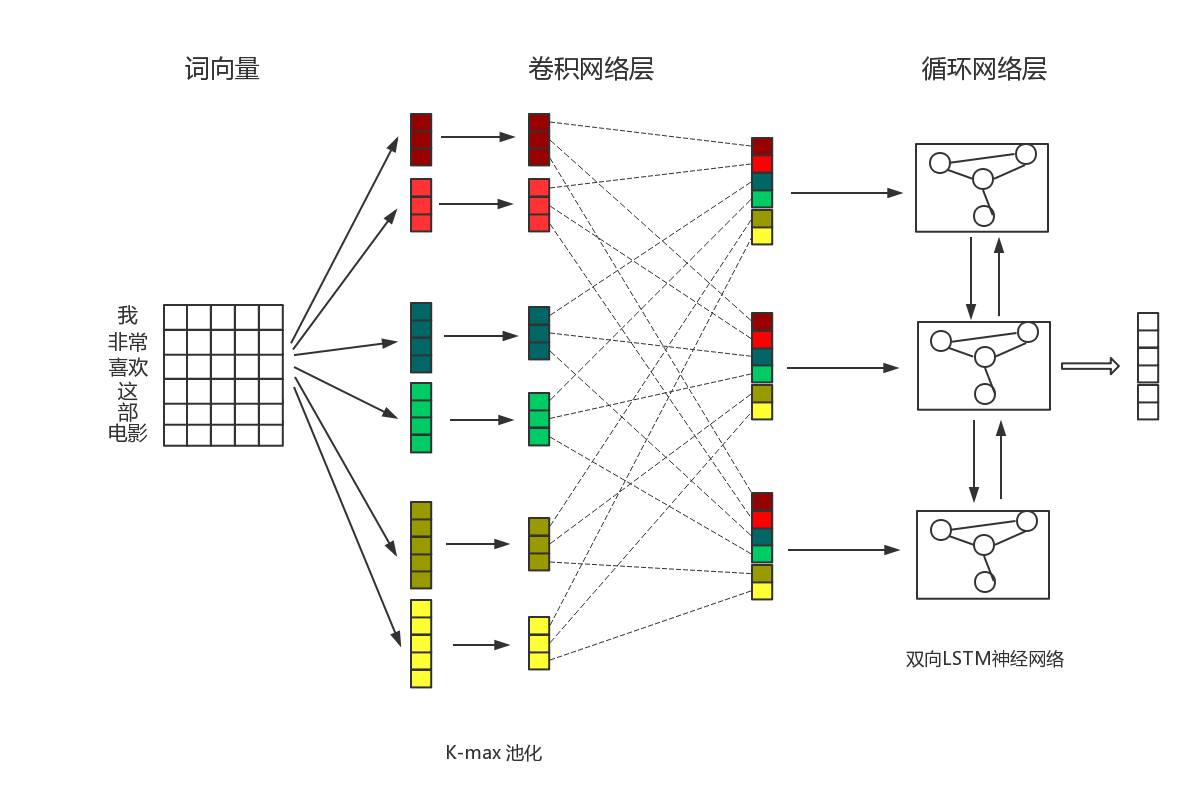
\includegraphics[scale=0.4]{picture/CLSTM.png}
    \caption{卷积循环神经网络结构图}
    \label{CLSTM}
\end{figure}
\subsection{卷积网络层}
卷积网络层的结构与普通卷积神经网络大致相同,分为卷积模块、池化模块与光栅模块。
为了适应本文研究的中文短文本数据,本文对每个模块的具体实现做出了一些调整,下面
对各个模块进行说明:

(1)卷积模块

基于文本数据的信息特征,卷积网络层的卷积模块使用窄卷积(Narrow Convolution)
作为卷积策略,避免宽卷积(Wide Convolution)的补零操作对提取文本特征造成影响。
卷积核长度分为3、4、5三种,宽度为词向量的长度,滑动步长为1,保证特征图能够包含尽可能多的文本特征。
每种卷积核生成128个,保障特征图的多样性。

(2)池化模块

由于短文本数据的长度以及卷积核的长度并不统一,卷积层产生的特征图的长度各有不同,
为了让接下来的循环网络层能够处理特征图,需要在池化模块对其进行处理,将长度统一。
本文使用k-max池化(k-max pooling)作为
池化算法,该算法是Kalchbrenner提出的动态k-max算法的前置算法\citing{kalchbrenner2014convolutional},
主要思想是对于一个给定的$k$值与特征序列$p$($p\in R^p,length(p)\geq k$),选择序列$p$中前$k$个最大值,
且保留原来序列的次序(即生成序列是原序列$p$的一个子序列)。通过k-max池化算法,卷积网络层不仅能够
接收变长的输入,同时生成的特征图也保留了相对的位置信息,提升了特征的质量。

(3)光栅模块

光栅模块主要用来整合生成的各个特征图,将其中相同位置的特征值进行合并,形成最终的特征向量,输入下面的循环网络层,
如网络结构图\ref{CLSTM}中的虚线所示。

\subsection{循环网络层}

循环神经网络依据时间对序列数据进行建模,上一个节点的数据不仅会进行输出,还会作为同一隐藏层下一个节点的输入,
隐藏层最后一个节点则能够接收到全部的文本特征数据。但是短文本分类任务需要更多的考虑文本上下文信息,单纯使用正向
循环神经网络,模型只能够依据上文信息进行分类,无法利用下文的信息,从而影响最终的分类效果。因此,本文使用
双向长短时记忆循环神经网络(Bi-directional Long Short-Term Memory,Bi-LSTM)作为循环网络层的实现,
将网络分为前向传递层与后向传递层,分别获取输入短文本的上文信息与下文信息。

Bi-LSTM网络的整体流程如图\ref{Bi-LSTM}所示,对于从上层网络传来的输入向量,网络首先将其转变为
正序序列及逆序序列两个向量,然后分别输入一个单向LSTM网络进行特征提取,得到正序特征向量与逆序特征向量,
之后将两个特征向量合并,形成最终的文本特征向量并输出到下一层网络。经过这样的处理,网络提取的特征向量既包含
上文信息又包含下文信息,能够给之后的分类网络提供更加丰富的语义信息,有效缓解了短文本数据语义信息不足的问题
,提升了分类的准确率。
\begin{figure}[h]
    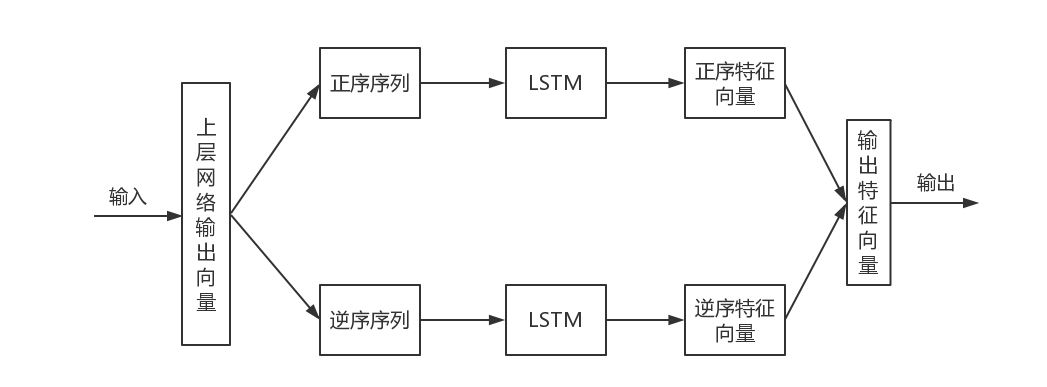
\includegraphics[scale=0.4]{picture/Bi-LSTM.png}
    \caption{Bi-LSTM网络流程图}
    \label{Bi-LSTM}
\end{figure}

\section{Attention Model}
Attention Model(注意力机制)是近几年兴起的一个新型模型,在很多场景被证明有效。
模型以认知心理学中的人脑注意力理论为核心,认为人脑在处理具体任务时,对于相关事物的注意力会集中在
某一个特定的地方,忽略其他无关的地方,而不是对每个地点分配相同的注意力。
通过这样的理论,Attention Model
能够合理的分配模型的计算资源,并且还可以避免非关键数据对结果的影响。
Attention Model最先在计算机视觉领域被
应用于图片识别等问题,取得了很好的成果,随后在自然语言处理领域也获得了优秀的成绩。
下面将以编码-解码模型中的Attention机制为例,
说明Attention Model的基本知识,然后在下一小节把Attention Model应用在卷积循环
神经网络当中。

编码-解码模型是自然语言处理领域中一个非常普遍的模型,它通过编码器将输入向量编码为中间
变量,再用解码器解码成输出向量,完成输入数据到另一组输出数据的转变,
从而实现多种内容转换任务,如机器翻译、文本复述等。
同时编码-解码模型的编码器与解码器没有具体限定,可以使用
各种各样的深度学习模型,如CNN、RNN等,让模型具有很强的泛用性,能够适合各种应用场景。
编码-解码模型的一般架构如图\ref{Encoder}所示。
\begin{figure}[h]
    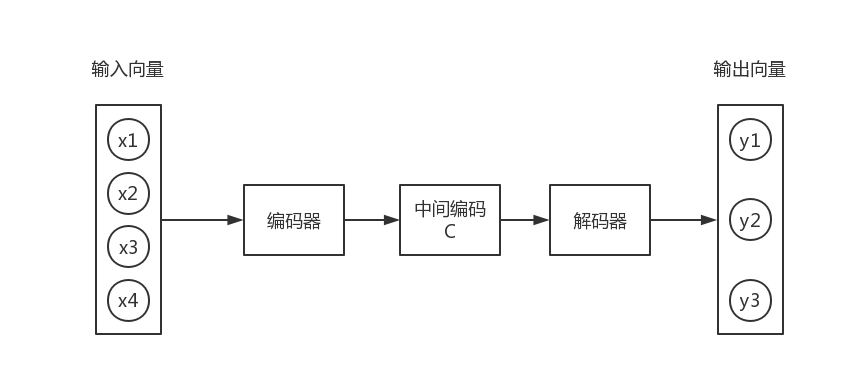
\includegraphics[scale=0.5]{picture/Encoder.png}
    \caption{编码-解码模型架构图}
    \label{Encoder}
\end{figure}

编码-解码模型的输入一般是一个长度为$n$向量序列$X$($X= \left \{x_1,x_2,x_3,...,x_n \right \}$),
输出则是一个长度为$m$的向量序列$Y$($Y= \left \{y_1,y_2,y_3,...,y_m \right \}$)。
模型运行时,编码器根据一定的映射规则对输入序列进行编码,得到中间编码$C$,表达公式如\ref{encode_eqn}所示。
\begin{equation}
    C=Encode\left ( x_1,x_2,x_3,...x_n \right )
    \label{encode_eqn}
\end{equation}
之后解码器对中间编码$C$进行解码,得到输出序列$Y$,计算公式如\ref{decode_eqn}所示。
\begin{equation}
    y_i=Decode\left ( C,y_1,y_2,y_3,...,y_{i-1} \right ),i=1,2,3,...,m
    \label{decode_eqn}
\end{equation}

可以看出解码器在计算输出序列$Y$时,对于每一个输出子项$y_i$用到的数据信息是一样的,都是
输入序列$X$编码后得到的中间编码$C$,
即输入序列$X$对输出序列$Y$中每一个子项的影响是相同的。这样的方式无疑忽略了
很多细节,在一些任务中甚至直接影响了输出结果。比如机器翻译任务,
一个词的翻译虽然与上下文和词本身同时有关,但对于人名机构名等名词,
翻译时词本身的影响必定较重,而其他的动词形容词等则可能上下文的影响较大,所以简单
输入序列同比例的作用在输出序列之上并不是一个好的方法。

Attention Model的出现很好的解决了这个问题,在Attention-Based编码-解码模型中,
编码器的输出不再是一个完整的中间编码$C$,而是输入序列$X$在编码阶段的历史状态$C_i$,
如公式\ref{attention_encode_eqn}所示。
\begin{equation}
    C_i=\sum_{j=1}^{n}\alpha_{ij}Encode\left ( x_j \right )
    \label{attention_encode_eqn}
\end{equation}
其中$\alpha_{ij}$表示当前输入子项$x_j$的注意力权重,这个值越高,表明$x_j$对结果
越重要。

解码器根据历史状态$C_i$得到优化后的输出序列,如公式\ref{attention_decode_eqn}所示。
\begin{equation}
    y_i=Decode\left ( C_i,y_1,y_2,y_3,...y_{i-1} \right ),i=1,2,3,...,m
    \label{attention_decode_eqn}
\end{equation}

可以发现,Attention Model本质上既是在模型的输出结果上添加一个注意力权重,
筛选对结果重要的数据项,同时过滤对结果影响较低的数据项,以此优化模型的输出效果。
这一思想在短文本分类任务中同样适用,因为对于短文本文本分类任务,确定分类结果的
往往是文本的几个关键词,如情感分析中的“喜欢”、“讨厌”等词,如果能够判断出这些关键词,
就可以极大的增强分类模型的结果。

\section{Attention-Based字词结合卷积循环中文短文本分类网络}
\subsection{Attention-Based卷积循环特征提取网络}
根据Attention Model的思想,
本文改进了\ref{CLSTM_section}小节提出的卷积循环特征提取网络,
增加注意力权重,优化原始网络产生的特征向量。

Attention Model的核心在于注意力权重的获取,有多种实现方式,如Soft Attention、
Hard Attention等\citing{xu2015show}。为了减少模型的计算负担,
本文选择参数化的Soft Attention实现方式,该实现方式能够让整个Attention层直接嵌入
模型,使梯度可以经过Attention Mechanism模块,反向传播到其他地方,以此简化模型的训练过程。
总体计算流程如图\ref{Soft_Attention}所示,
首先把双层LSTM的输出$h$($h=\left \{ h_1,h_2,..,h_n\right\}$)
送入一个单层全连接神经网络,根据\ref{attention_eqn1}公式将其转换为中间向量$u$,
作为原始输出$h$的隐藏表示。
\begin{equation}
    u_i=\tanh\left ( W_wh_i+b_w \right )
    \label{attention_eqn1}
\end{equation}

然后通过softmax函数计算中间向量$u$与文本上下文向量$u_w$的相似度$\alpha$,如公式\ref{attention_eqn2}所示。
\begin{equation}
    \alpha_i=\frac{\exp\left ( u_{i}^{\top }u_w \right )}{\sum_n\exp\left ( u_{i}^{\top }u_w \right )}
    \label{attention_eqn2}
\end{equation}

其中$u_w$是记忆向量,可以视为筛选重要特征的高层抽象参数,代表着
整个语料库的上下文信息\citing{sukhbaatar2015end},在模型初始阶段随机初始化,
并在训练时同其他参数一起调整。计算结果$\alpha$则是标准化的注意力权重,用于下一步计算。

最后,把原始向量$h$和$\alpha$加权相加,就得到Attention优化后的特征向量$S$,如公式\ref{attention_eqn3}所示。
\begin{equation}
    S_i=\sum_n\alpha_ih_i
    \label{attention_eqn3}
\end{equation}
\begin{figure}[h]
    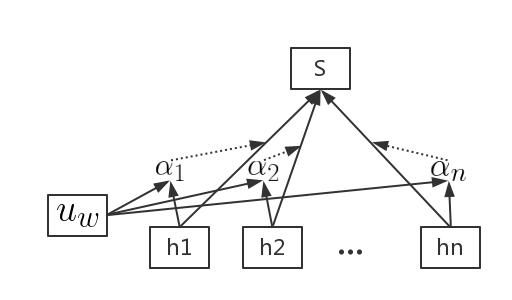
\includegraphics[scale=0.5]{picture/Attention.png}
    \caption{Soft Attention计算流程}
    \label{Soft_Attention}
\end{figure}

\subsection{双通道字词结合短文本分类模型}
在短文本分类任务中,词向量与字向量都能够作为文本的向量表示,但都有其固有的缺点:
词向量极度依赖分词结果,错误的分词会极大的影响词向量的性能;字向量虽然不存在分词的问题,但有些词语和
内部的汉字意思可能南辕北辙,如“东西”与其内部的汉字“东”和“西”,单纯从字向量很难推测出词的含义。
为了解决这个问题,本文设计了双通道字词结合短文本分类模型,同时接受短文本的词向量表示与字向量表示,
充分结合两者的特征信息,克服了常规分类模型的不足。

\begin{figure}[h]
    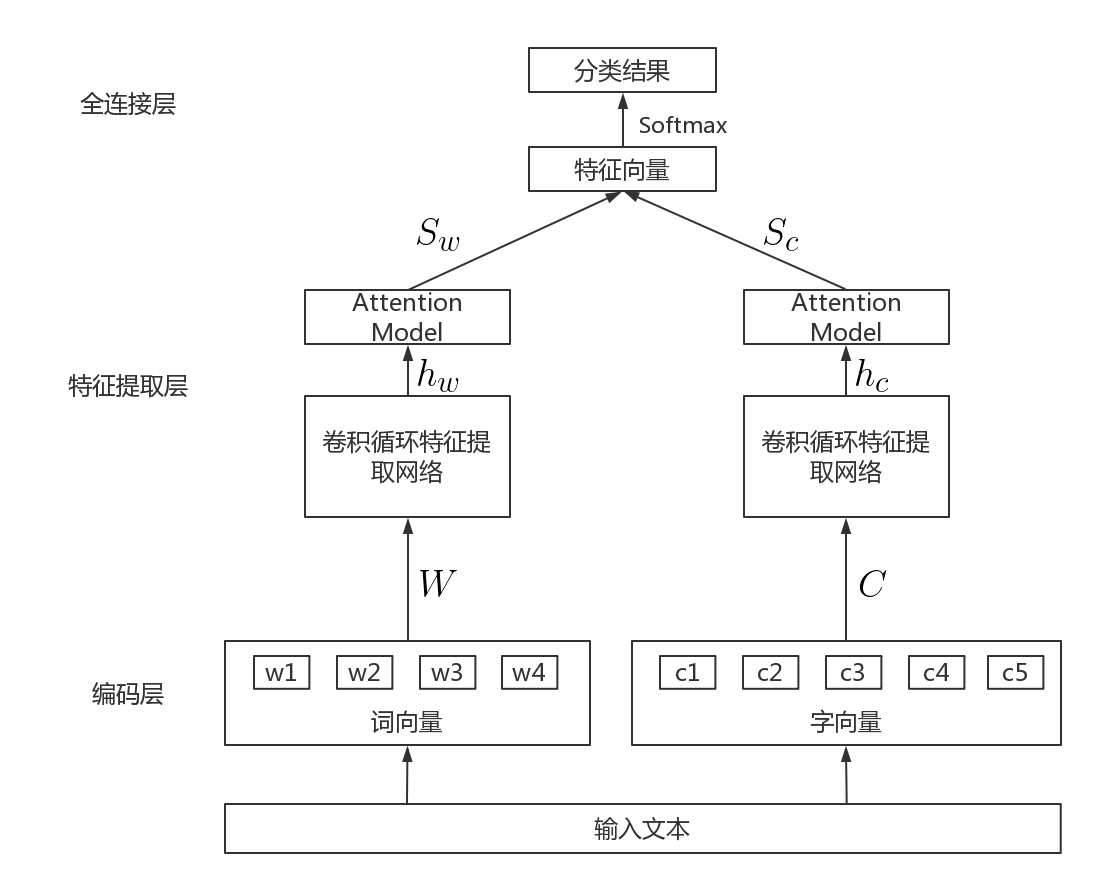
\includegraphics[scale=0.4]{picture/classifier.png}
    \caption{双通道字词结合短文本分类模型}
    \label{classifier}
\end{figure}

双通道字词结合短文本分类模型主要是构建一个包含两个平行的特征提取网络的分类模型,分别提取词向量特征与字向量特征,
总体结构如图\ref{classifier}所示。

模型总共分为三层:编码层、特征提取层与全连接层。编码层根据相应的词向量与字向量模型,将输入文本解析为词向量序列$W$
和字向量序列$C$。特征提取层分为两个平行的神经网络模块,由前文中的Attention-Based卷积循环特征提取网络组成,
分别提取词向量序列和字向量序列的文本特征,即向量$S_w$、$S_c$,然后根据公式\ref{classifier_eqn}将其合并,得到最终的文本特征向量$S$。
\begin{equation}
    S =\left [ S_w\bigoplus S_c \right ]
    \label{classifier_eqn}
\end{equation}

全连接层由线性转换层和Softmax层组成,其中线性转换层将特征向量$S$转换为一个维度与分类类别相当的实值向量,然后
Softmax层将这些实值映射为最终的条件概率,计算公式如\ref{softmax_eqn}所示。
\begin{equation}
    P=softmax\left ( W_sS+b_s \right )
    \label{softmax_eqn}
\end{equation}

对于模型训练,本文使用公式\ref{cost_function}作为模型的损失函数,来最小化模型的分类误差。其中$N_t$表示训练语料库大小,
$N_c$表示类别数量,$P_{j}^{g}\left ( s_i \right )$表示当前文本的真实类别为$j$的概率,属于类别$j$则为1,否则为0。
并且使用随机梯度下降算法(Stochastic Gradient Descent,SGD)作为训练的优化算法。
\begin{equation}
    Loss=-\sum_{i=1}^{N_t}\sum_{j=1}^{N_c}P_{j}^{g}\left ( s_i \right )\cdot\log\left ( P_j\left ( s_i \right ) \right )
    \label{cost_function}
\end{equation}
\section{实验结果和分析}
\section{本章小结}